\scanpage{58}
par $\Sigma$, muni d'une stratification locale
cylindrique ordonnée : $\Sigma'(1)$ est l'espace des
strates de codim $1$, $\Sigma'(1)\overset{\uline{b}}{-}\Sigma\unsure{{}_{0}|.}$ l'application
associant à un germe son centre, $\Sigma'(2)$ est
l'espace des paires de germes $B,B'$ en $x$
\deleted{\unsure{que}} tels que : $\{B\}<\{B'\}$ \unsure{...|\illegible{1}..}
\margin{\diagram{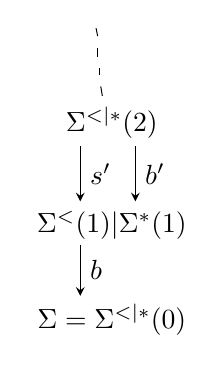
\begin{tikzpicture}[x=1cm,y=1cm,>=stealth]
\draw[line width=.35pt] (-.2,1.65)--(-.18,1.55);
\draw[line width=.35pt] (-.18,1.4)--(-.18,1.28);
\draw[line width=.35pt] (-.16,1.14)--(-.16,1.06);
\draw[line width=.35pt] (-.14,.91)--(-.12,.79);
\node at (0,.45) {$\Sigma^{\unsure{<|*}}(2)$};
\node at (0,-.85) {$\unsure{\Sigma^{<}(1)|\Sigma^{*}(1)}$};
\node at (0,-2.05) {$\Sigma=\Sigma^{\unsure{<|*}}(0)$};
\draw[->] (-.4,.15)--(-.4,-.55) node[midway,right] {$\uline{s}'$};
\draw[->] (.3,.15)--(.3,-.55) node[midway,right] {$\uline{b}'$};
\draw[->] (-.4,-1.1)--(-.4,-1.75) node[midway,right] {$\uline{b}$};
\end{tikzpicture}}}
Pour retrouver la relation d'ordre sur $\Sigma\unsure{=|\substack{-\\0}}\Sigma^{\unsure{<|*}}(0)$
\inserted{à partir de la structure d'ordre relative $\Sigma^{\unsure{*|<}}(1)$ sur $\Sigma^{<}(0)$ (celle
qui \unsure{place} $\Sigma^{<}(1)$ pour les relations strictes $x<y$)}
il faut donc de plus se donner une application
continue
\[
(36)\qquad\Sigma^{<}(1)\overset{\uline{s}\unsure{=|:}p_1}{-}\Sigma_{\deleted{\unsure{*|\varnothing|0}}}=\Sigma^{<}(0)
\]
qui soit injective \deleted{et croissante} sur chaque fibre \inserted{$\uline{b}^{-1}(x)$}
de $\Sigma^{<}(1)\overset{\uline{b}}{-}\Sigma_{\deleted{\unsure{*|\varnothing|0}}}$ (i.e. $\Sigma^{<}(1)\overset{(\uline{s},\uline{b})}{-}\Sigma\times\Sigma$ inj.)
et d'image $\not\ni x$ (i.e. $\operatorname{Im}(\uline{s},\uline{b})\cap\operatorname{diag}(\Sigma\times\Sigma)=\varnothing$)

\deleted{et on doit se donner de plus
\[
(37)\qquad\Sigma^{<}(2)\xrightarrow{\unsure{\varphi_2|p_2}}\Sigma^{*}(1)\quad(\hookrightarrow\Sigma\times\Sigma
\]
\margin{NB la donnée de $\unsure{\varphi_2|p_2}$ équivaut à celle des deux composés
$\operatorname{pr}_{\unsure{0|1}}\circ\varphi;\operatorname{pr}_{\unsure{1|2}}\circ\varphi:\Sigma^{<}(2)\rightrightarrows\Sigma$
qu'on \unsure{se} donne}
\margin{inutile de se donner $p_2$, il est déterminé ($v\ p_1$), cf \unsure{pg} suivante\unsure{..|.-|...}}
\[
(38)\qquad
\Sigma^{<}(2)\xrightarrow{(\operatorname{pr}_1\circ\varphi,\operatorname{pr}_2\circ\varphi,\unsure{\Psi|\psi})}\Sigma_0\times\Sigma_0\times\Sigma_0
\]
\unsure{\deleted{Dont}|Dont} l'image est par construction (voir \unsure{\deleted{\varphi}|\varphi|\illegible{1}} (37))
dans $\Sigma_1\times\Sigma_0$ et dans
}
\margin{\handwritten{57}}
